\chapter{Repository Deep Dive}\label{chap:Repository_Deep_Dive}
\section{Verilator Simulator}\label{sec:Verilator_Simulator}
\subsection{About}\label{sec:About_Verilator_Simulator}
The primary way to simulate SoCs' designed using the Chipyard framework is via Verilator simulations.
The directory for verilator is \file{chipyard/sims/verilator}.
An example simulation can be run by using \mintinline{bash}{make} in the verilator directory.
Running the \texttt{make} command produces a simulator executable in the verilator directory.

Custom Chipyard configs can be simulated by running \mintinline{bash}{make CONFIG=<your custom config>}.
For example, if your project name was ``TestConfig'', running \mintinline{bash}{make CONFIG=TestConfig} would create an executable called \file{simulator-chipyard-TestConfig} in the \file{verilator} directory.
Custom RISCV code can be run by using the command \mintinline{bash}{./simulator-chipyard-TestConfig /path/to/riscv/executable} from the \file{chipyard/sims/verilator} directory.

\subsection{Generators}\label{sec:Generators}
\subsubsection{Chipyard Generator}\label{sec:Chipyard_Generator}
\subsubsection{SHA3 Accelerators}\label{sec:SHA3_Accelerators_Generator}

\subsection{Custom Configurations}\label{sec:Custom_Configurations}
Custom Configs can be created in the directory \mintinline{bash}{chipyard/generators/chipyard/src/main/scala/config/}.
For example, I created a new scala file called \file{NewTestConfig.scala} in the directory, allowing me to create a simulator from a class inside the NewTestConfig.scala file.
Example Configs can be found in  \file{RocketConfigs.scala} in the same directory.

% Include custom config example


\subsection{FPGA Implementation}\label{sec:FPGA_Implementation}


\subsubsection{About}\label{sec:About}

\begin{figure}[h!tbp]
  \centering
  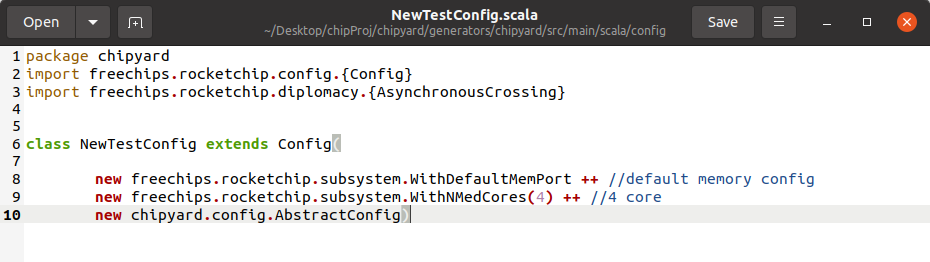
\includegraphics[width=0.7\linewidth]{./NewTestConfig.png}
  \caption{\file{NewTestConfig.scala}}
  \label{fig:newtestconfig}
\end{figure}

%%% Local Variables:
%%% mode: latex
%%% TeX-master: "../doc"
%%% End:
